\chapter{Privacy Leaks with JPEG Digital Photographs}\label{ch-jpeg}

\hl{This chapter needs to be refactored to simply describe the JPEG
  format, present a tool that shows the hidden information, then
  briefly describe how to go deeper.}

A digital photograph is nothing more than a collection of
pixels that, when viewed by a human, seems to resemble something that
might be seen with the human eye. Different approaches to digital
photography date back to the 1970s, when large grey-scale photographs
were printed on long reams of paper with teleprinters and hung in
computer centers. Up close these printouts looked like
gibberish. Viewed from a distance, they resembled black-and-white photographs.

Modern digital photography is the result of three enabling
technologies: low-cost lenses and sensor that can capture
high-resolution imagery; screens, that allow for both the preview and
final display of the images; and high-quality compression algorithms,
that make it possible to shrink the data captured by the sensors to a
more convenient size for transportation and storage.

This chapter concerns itself with data leaks resulting from the JPEG
file format, a popular compression algorithm. It is hard to understate
the importance of JPEG. Prior to its introduction, digital images were
large. An 8-bit black-and-white photo for a standard video resolution
of 640-by-480 pixels was 307,200 bytes; a full-color photo required
three times that much, nearly a megabyte of data. JPEG made it
possible to compress a full-color image to a tenth of its original
size without any noticable loss in quality, and to be compressed to a
twentieth while still looking quite good.

It is hard to overstate the impact that low cost digital photography
has had on our planet. Just two decades ago, the act of making a
picture was a relatively rare and special event. Most people did not
carry cameras---those people who did frequently stood out. Cameras
were frequently viewed with suspicion. Most events were not visually
recorded. Today matters are reversed in much of the world. There are
now more activated smartphones and camera-enabled feature phones than
human beings on much of the
planet\footnote{\url{http://www.ctia.org/advocacy/research/index.cfm/aid/10323}}\footnote{\url{http://en.wikipedia.org/wiki/Mobile_phone_penetration_rate}}. As
a result, many events that once would have been lost to history or
memory are now visually recorded---sometimes covertly---and those
recordings can be redistributed to millions of people with
ease. Photographs and videos made by bystanders have had profound
impact on many world events.

\sgraphic[width=3in]{ch-jpeg/settled.png}{Reprinted under the Creative
  Commons license from \url{http://xkcd.com/1235}}

This chapter is not about the ability of digital photographs and
videos to violate privacy based on their overt content. This chapter
will also not discuss \emph{steganography}, in which secret messages
are intentionally hidden in the image data.

Instead, this chapter is about the ability of digital media to
inadvertently reveal private information without the realization of
the photographer or publisher.  The first section of this chapter
describes the JPEG format itself. JPEG files are built from a series
of binary sections or \emph{chunks}. One kind of section are JPEG
thumbnails; in the second section we'll see a variety of ways that
thumbnails can leak private information. Section~\ref{sec:exif}
discusses the Exif format, which is a way for structuring JPEG
metadata. The last section looks at some non-obvious ways that the
content of JPEGs themselves can leak information.

\section{The JPEG file format}

The most common digital image compression format in use today is the
JPEG File Interchange Format (JFIF) and the Exchangeable image file
format (Exif). The name ``JPEG'' stands for the Joint Photographic Experts
Group, an international committee that was formed in 1986 to develop digital
photography standards.  The JFIF standard was released in 1992 and was
widely adopted because of its technical capabilities; the Exif
standard, released in 1995, extended the JPEG standard by adding the
ability to store metadata directly in the file such as the date and
time that the photo was taken, camera settings, and other
information. In this chapter we will follow colloquial usage and refer
generically to files in the JFIF or Exif format as ``a JPEG.'' They
are typically given the file extension \emph{.jpg} or \emph{.jpeg},
although \emph{.jif} and \emph{.jfif} are also used. JPEG files can
also be put directly into a database as a BLOB (binary large
object), in which case they really just a sequence of bits with neither a file name nor an extensions.

JPEG is a \emph{tunable, lossy} compression algorithm: when an image
is compressed and then decompressed with JPEG, the resulting image is
different from the original (hence the ``lossy''). How different depends on the amount of
compression specified (the ``tunable'' part). The ImageMagick |convert| program allows images
to be resized and compressed in a single operation; the compression
amount is typically specified as a number between 1 (maximum compression) and 100;
\figref{jpeg-sizes} shows the same image with compressions of 10, 50,
and 99.

\begin{figure}
\begin{tabular}{ccc}
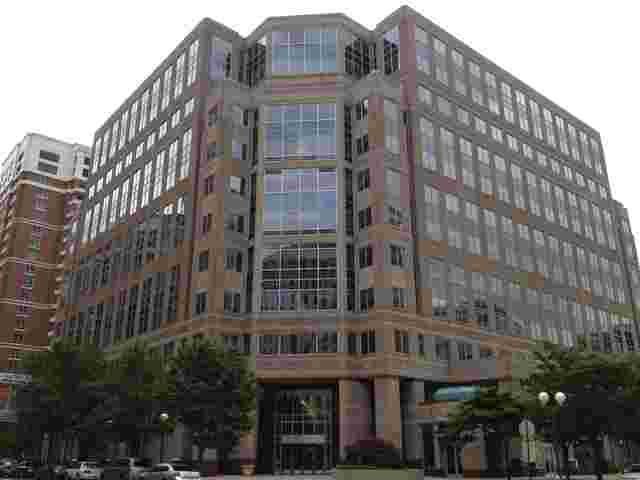
\includegraphics[width=2in]{ch-jpeg/nsf_hq_640x480-q10.jpg} & 
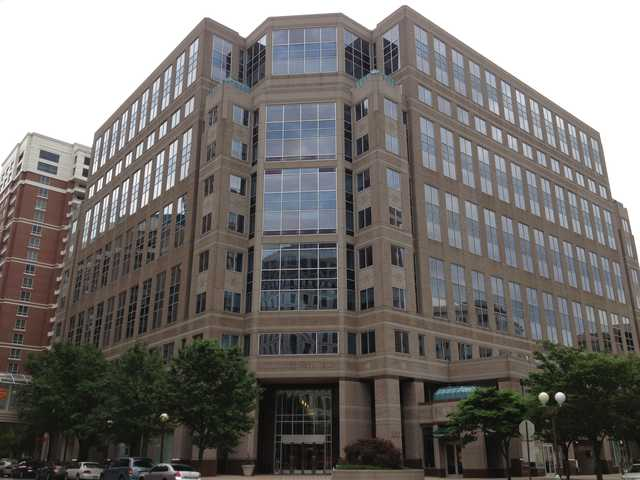
\includegraphics[width=2in]{ch-jpeg/nsf_hq_640x480-q50.jpg} &
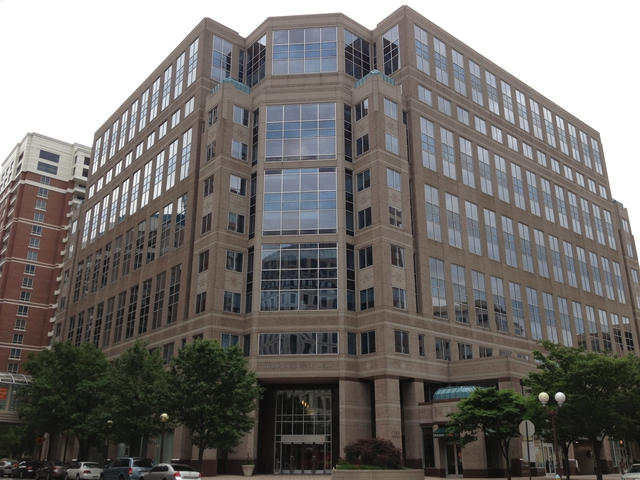
\includegraphics[width=2in]{ch-jpeg/nsf_hq_640x480-q100.jpg} \\
Quality 10 & Quality 50 & Quality 100 \\
23,422 Bytes & 49,305 Bytes & 248,279 bytes \\
1:40 compression & 1:18 compression & 1:4 compression\\
\end{tabular}
\caption{A test image showing three JPEG compression rates. Each image
  is 640x480 pixels. The original uncompressed image required 921,600 bytes.}
\end{figure}

The JPEG file itself is structured as a series of \emph{segments} that are
concatenated together. Each segment begins with a \emph{marker}
consisting of a |FFh| followed by a single-byte code and a data payload. Some segments are fixed
length while others variable size. Typically variable-signed markers
are used for image data or variable-length metadata. The marker
types are described in \tabref{tab:jpeg-format}. Exif metadata is stored in the APP2
segment type, which itself contains its own series of tagged
segments. 

% http://stackoverflow.com/questions/2270082/latex-how-do-i-change-the-font-size-of-a-table-column

\begin{table}
\begin{tabularx}{\textwidth}{l>{\tt}l>{\it}clX}
       & \rm Segment &         &      & \\
Abbrev & \rm Marker  & Payload & Name & Comments\\
\hline
\hline
SOI  & FF D8 &        - & Start of Image & Beginning of file \\
\hline
\hline
APP0 & FF E0 &  $>16$   & JFIF APP0                        & \\
\hline
APP1 & FF E1 & variable & APP1                             & Exif Metadata\\
\hline
APP14 & FF EE & variable & APP14 & Copyright Information\\
\hline
APP\it{n} & FF E\it{n}& - & Application specific           & Other extensions; not widely used\\
\hline
\hline
SOF\it{n} & FF C\it{n} & variable & Start of frame \emph{n}& Start of coding-specific information\\
\hline
SOF0 & FF C0 & variable & Start of Frame (Baseline DCT)    & Also specifies the width, height, number of components, and component subsampling. \\
\hline
SOF2 & FF C2 & variable & Start of Frame (Progressive DCT) & Also specifies the width, height, number of components, and component subsampling. \\
\hline
DHT  & FF C4 & variable & Define Huffman Tables(s)         & Huffman tables follow.\\
\hline
\hline
DQT  & FF DB & variable & Define Quantization Table(s)     & Quantization tables follow.\\
\hline
DRI  & FF DD & 2 bytes  & Define Restart Interval          & Specifies interval between RST\emph{n} markers in macroblocks.\\
\hline
SOS  & FF DA & variable & Start of Scan                    & Image data follows, top-to-bottom scan of image. Progressive DCT JPEGs may contain multiple scans.\\
\hline
RST\it{n} & FF D\it{n}& - & Restart                        & Restart specified by DRI marker.\\
\hline
COM & FF FE & variable  & Comment                          &   Contains comment text\\
\hline
EOI & FF D9 & -         & End of Image\\
\hline
\hline
\end{tabularx}
\caption{JPEG marker types, from
  \url{https://en.wikipedia.org/wiki/JPEG} and
  \url{http://de.wikipedia.org/wiki/JPEG_File_Interchange_Format},  with modifications. Note
  that bytes are in hex.}\label{tab:jpeg-format}
\end{table}

One of the challenges in developing file formats is assuring
\emph{backward compatability} so that newer versions of the files will
be readable by old software that hasn't been updated. JPEG's
segment-based file format is designed to allow backward compatibility:
software that doesn't know how to read a particular segment should, in
theory, be able to just skip over it. In order to do this skip the
software needs a way to find the next segment. JPEG provides two
mechanisms. First, the length of variable-length segments is encoded
in the first two bytes after the marker: if the marker begins \texttt{FFh xx
  s1 s2}, \texttt{FF xx} denotes the segment type and the length
is $256 \times \texttt{s1} + \texttt{s2}$. Second, the character |FFh|
denotes the start of a segment; when |FFh| needs to appear in binary
data, the JPEG standard calls for the value to be entered into the
file as the sequence |FFh 00h|.

From this brief introduction to the standard we can see that there are  several places where
data other than image data might be present in a JPEG file:

\begin{enumerate}
\item After the EOI marker
\item Inside Comment segment
\item Inside the Exif metadata segment
\end{enumerate}

\subsection{A program to validate JPEGs}

To find this kind of information we need a program that understands
the JPEG file format. Many such programs exist, but few of them allow
the degree of control that we require here. Therefore we will present
a short program that understands a small amount of the format and use
it to find the examples of the first two above. The Exif format is
rather complicated, however, so we'll use a specialized open source
tool for that one.

\lstinputlisting[caption=A simple Python program for decoding the JPEG file structure,label=jpeg_scan]{ch-jpeg/jpeg_scan.py}

Listing~\ref{jpeg_scan} is a simple python program that understands
the basic structure of the JFIF and Exif file format. The main
function is |validate_jpeg(fn)|, which opens the named file, reads it
into a buffer called |data|, and then loops through the JFIF
segments. The body of this function is the |while| loop, which checks
to make sure that it has a marker (beginning with a |FF|). It
dispenses with the fixed size segments, provides special handling for
the SOS segment (which extends to the end of the file), and then has
handling for the variable-length segments (the program assumes that
any unknown marker is going variable-length). As an example of
handling variable-sized programs the program prints comments.

Following the function is the part of the program that parses
arguments. If one or more files are provided, they are processed. If a directory name is provided, the program iterates
through all subdirectories, looking for a files with extensions ending
in \emph{.jpg} or \emph{.jpeg}. The debug option causes
\emph{validate\_jpeg()} to print the location and codes of all of the segment markers.

Below is an example of the output that this program produces:

\begin{Verbatim}
output
\end{Verbatim}

We ran this program on several hundred thousand files to look for
JPEGs with anomalous contents. The following sections describe some of
what we found.

\subsection{Files that are not JPEGs}

Files that do not begin with the JPEG ``magic number'' of |FF D8|
cannot be JPEGs. In many cases we found files in other image file
formats---most notably PNG and TIFF. Double-clicking one of these
files will will typically cause the program that is registered to
display JPEG images to attempt to display the file; whether or not the
file actually displays depends on the program. 

\subsection{Data at the end of the JPEG}

One place where information can be hidden is after the JPEG's EOI
marker but before the file's end. This approach hides the data because
programs that display JPEGs stop when they encounter the end of the
image.  

Scanning through the images that we've seen with data after the EOI,
we have found:

\begin{itemize}
\item In a JPEG that was copied from a web page, there were fragments
  of the HTML table that surrounded the image.
\item On a series of photos taken with a Nokia Lumia 822 cellular phone,
  there was 32 character hexadecimal string (128 bits).
\item On a photo taken with an HTC Android phone, there was more than
  10 kilobytes of high entropy data.
\end{itemize}


\begin{lstlisting}[caption={A 40-character block of text consisting of
    two dashes, a 128-bit string (32 hexadecimal
    numbers), two more dashes, a carriage return and a line feed were
    found at the end of every photo taken with a Nokia Lumia 822
    cellular phone. Is this a serial number?},label=lumia822]
--5D9144052FC54aa482D8595FB8D52F1D--
\end{lstlisting}

\subsection{Data in the JPEG Comment}

The JPEG COM Marker introduces comment text that may be up to 64KiB in
length. We analyzed comments on discovered:

\begin{itemize}
\item Many JPEGs had comments indicating the programs that had created
  them. 
\item Apple's iPhoto application sets the Comment to be the same as
  the caption when a slideshow is created.
\end{itemize}

For example, many programs created with the The Gnome Image Manipulation
Program (The GIMP) had comments indicating ``Created with the
GIMP''. It turns out that The GIMP sets this field by default, but it
is only evident when the ``Advanced'' settings of the ``Export'' panel
are exposed.

Comments that reveal the program used to create the image make it
possible to link together multiple images that came from the same
person (although the linkage is unreliable and easily forged). Because
comments may not be removed if an image is edited, they may cause
information to be leaked from one use of a photo to another. 

\sgraphic{ch-jpeg/gimp_save_as}{The GIMP allows the user to specify
  the Comment of a JPEG''}

It turns out that there are several different ways to crop JPEG
photographs on the Macintosh computer that was used to make
\figref{ch-1/nsf_hq}. One of the programs is Apple's iPhoto, which has
check boxes for including ``Title and keywords'' and ``Location
information'' on its export dialog box. 

\bifigure{ch-1/export}{ch-1/export1}{Apple's iPhoto (left) allows the user to select whether or not
  titles and location metadata will be included in exported
  photographs; Apple's Preview tool (right) copies metadata without
  warning the user.}



\section{Exif metadata}\label{sec:exif}
By far the most revealing kinds of information is 

\subsection{Thumbnails}
\subsection{GPS Coordinates}
\subsection{Date and Time}
\subsection{Other Exif Information}

\section{Non-obvious image content information}
\subsection{Non-Subject Information Leakage}
\subsection{Reflections}
\subsection{Details in Shadows}
\subsection{High-Resolution Information}


